\begin{verbatim}


 [n, p, V, Fn, Fp, Jn, Jp, it, res] = secs1d_dd_gummel_map (x, D, Na, Nd, 
                                                       pin, nin, Vin, Fnin, 
                                                       Fpin, l2, er, u0n, 
                                                       uminn, vsatn, betan, 
                                                       Nrefn, u0p, uminp, vsatp, 
                                                       betap, Nrefp, theta, tn, tp, 
                                                       Cn, Cp, an, ap, Ecritnin, Ecritpin, 
                                                       toll, maxit, ptoll, pmaxit)         

 This function solves the scaled stationary bipolar DD 
 equation system using Gummel algorithm

     input: 
            x                        spatial grid
            D, Na, Nd                doping profile
            pin                      initial guess for hole concentration
            nin                      initial guess for electron concentration
            Vin                      initial guess for electrostatic potential
            Fnin                     initial guess for electron Fermi potential
            Fpin                     initial guess for hole Fermi potential
            l2                       scaled Debye length squared
            er                       relative electric permittivity
            u0n, uminn, vsatn, Nrefn electron mobility model coefficients
            u0p, uminp, vsatp, Nrefp hole mobility model coefficients
            theta                    intrinsic carrier density
            tn, tp, Cn, Cp, 
            an, ap, 
            Ecritnin, Ecritpin       generation recombination model parameters
            toll                     tolerance for Gummel iterarion convergence test
            maxit                    maximum number of Gummel iterarions
            ptoll                    convergence test tolerance for the non linear
                                     Poisson solver
            pmaxit                   maximum number of Newton iterarions

     output: 
             n     electron concentration
             p     hole concentration
             V     electrostatic potential
             Fn    electron Fermi potential
             Fp    hole Fermi potential
             Jn    electron current density
             Jp    hole current density
             it    number of Gummel iterations performed
             res   total potential increment at each step


\end{verbatim}




\subsection{Demo 1 for unction secs1d\_dd\_gummel\_map}
\begin{verbatim}

 % physical constants and parameters
 secs1d_physical_constants;
 secs1d_silicon_material_properties;
 
 % geometry
 L  = 10e-6;          % [m] 
 xm = L/2;
 
 Nelements = 1000;
 x         = linspace (0, L, Nelements+1)';
 sinodes   = [1:length(x)];
 
 % dielectric constant (silicon)
 er = esir * ones (Nelements, 1);
 
 % doping profile [m^{-3}]
 Na = 1e23 * (x <= xm);
 Nd = 1e23 * (x > xm);
 
 % avoid zero doping
 D  = Nd - Na;  
  
 % initial guess for n, p, V, phin, phip
 V_p = -1;
 V_n =  0;
 
 Fp = V_p * (x <= xm);
 Fn = Fp;
 
 p = abs (D) / 2 .* (1 + sqrt (1 + 4 * (ni./abs(D)) .^2)) .* (x <= xm) + ...
     ni^2 ./ (abs (D) / 2 .* (1 + sqrt (1 + 4 * (ni ./ abs (D)) .^2))) .* (x > xm);
 
 n = abs (D) / 2 .* (1 + sqrt (1 + 4 * (ni ./ abs (D)) .^ 2)) .* (x > xm) + ...
     ni ^ 2 ./ (abs (D) / 2 .* (1 + sqrt (1 + 4 * (ni ./ abs (D)) .^2))) .* (x <= xm);
 
 V = Fn + Vth * log (n / ni);
 
 % scaling factors
 xbar = L;                       % [m]
 nbar = norm(D, 'inf');          % [m^{-3}]
 Vbar = Vth;                     % [V]
 mubar = max (u0n, u0p);         % [m^2 V^{-1} s^{-1}]
 tbar = xbar^2 / (mubar * Vbar); % [s]
 Rbar = nbar / tbar;             % [m^{-3} s^{-1}]
 Ebar = Vbar / xbar;             % [V m^{-1}]
 Jbar = q * mubar * nbar * Ebar; % [A m^{-2}]
 CAubar = Rbar / nbar^3;         % [m^6 s^{-1}]
 abar = 1/xbar;                  % [m^{-1}]
 
 % scaling procedure
 l2 = e0 * Vbar / (q * nbar * xbar^2);
 theta = ni / nbar;
 
 xin = x / xbar;
 Din = D / nbar;
 Nain = Na / nbar;
 Ndin = Nd / nbar;
 pin = p / nbar;
 nin = n / nbar;
 Vin = V / Vbar;
 Fnin = Vin - log (nin);
 Fpin = Vin + log (pin);
 
 tnin = tn / tbar;
 tpin = tp / tbar;
 
 u0nin = u0n / mubar;
 uminnin = uminn / mubar;
 vsatnin = vsatn / (mubar * Ebar);
 
 u0pin = u0p / mubar;
 uminpin = uminp / mubar;
 vsatpin = vsatp / (mubar * Ebar);
 
 Nrefnin = Nrefn / nbar;
 Nrefpin = Nrefp / nbar;
 
 Cnin     = Cn / CAubar;
 Cpin     = Cp / CAubar;
 
 anin     = an / abar;
 apin     = ap / abar;
 Ecritnin = Ecritn / Ebar;
 Ecritpin = Ecritp / Ebar;
 
 % tolerances for convergence checks
 toll  = 1e-3;
 maxit = 1000;
 ptoll = 1e-12;
 pmaxit = 1000;
 
 % solve the problem using the full DD model
 [nout, pout, Vout, Fnout, Fpout, Jnout, Jpout, it, res] = ...
       secs1d_dd_gummel_map (xin, Din, Nain, Ndin, pin, nin, Vin, Fnin, Fpin, ...
                             l2, er, u0nin, uminnin, vsatnin, betan, Nrefnin, ...
 	                       u0pin, uminpin, vsatpin, betap, Nrefpin, theta, ...
 		               tnin, tpin, Cnin, Cpin, anin, apin, ...
 		               Ecritnin, Ecritpin, toll, maxit, ptoll, pmaxit); 
 
 % Descaling procedure
 n    = nout*nbar;
 p    = pout*nbar;
 V    = Vout*Vbar;
 Fn   = V - Vth*log(n/ni);
 Fp   = V + Vth*log(p/ni);
 dV   = diff(V);
 dx   = diff(x);
 E    = -dV./dx;
 
 % band structure
 Efn  = -Fn;
 Efp  = -Fp;
 Ec   = Vth*log(Nc./n)+Efn;
 Ev   = -Vth*log(Nv./p)+Efp;
 
 plot (x, Efn, x, Efp, x, Ec, x, Ev)
 legend ('Efn', 'Efp', 'Ec', 'Ev')
 axis tight
\end{verbatim}

\begin{figure}\centering
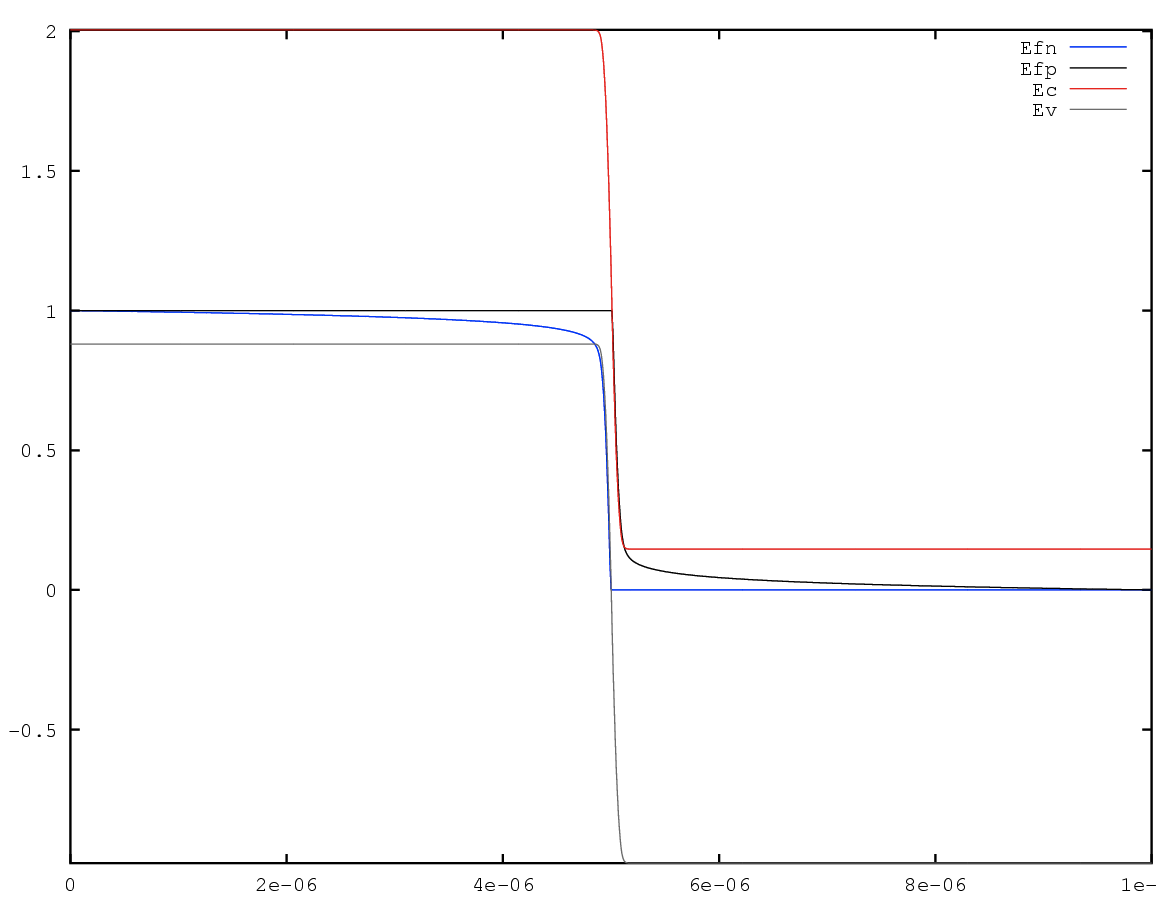
\includegraphics[width=.7\linewidth]{function/images/secs1d_dd_gummel_map_205.png}
\caption{Figure produced by demo number 1 for function secs1d\_dd\_gummel\_map}
\label{fig:secs1d_dd_gummel_map_figure_1}
\end{figure}
\clearpage
